% !TEX root = ../main.tex
\subsubsection{Cuts}
\label{12.41::cuts}
    \begin{figure}[b!]
        \centering\frame{
        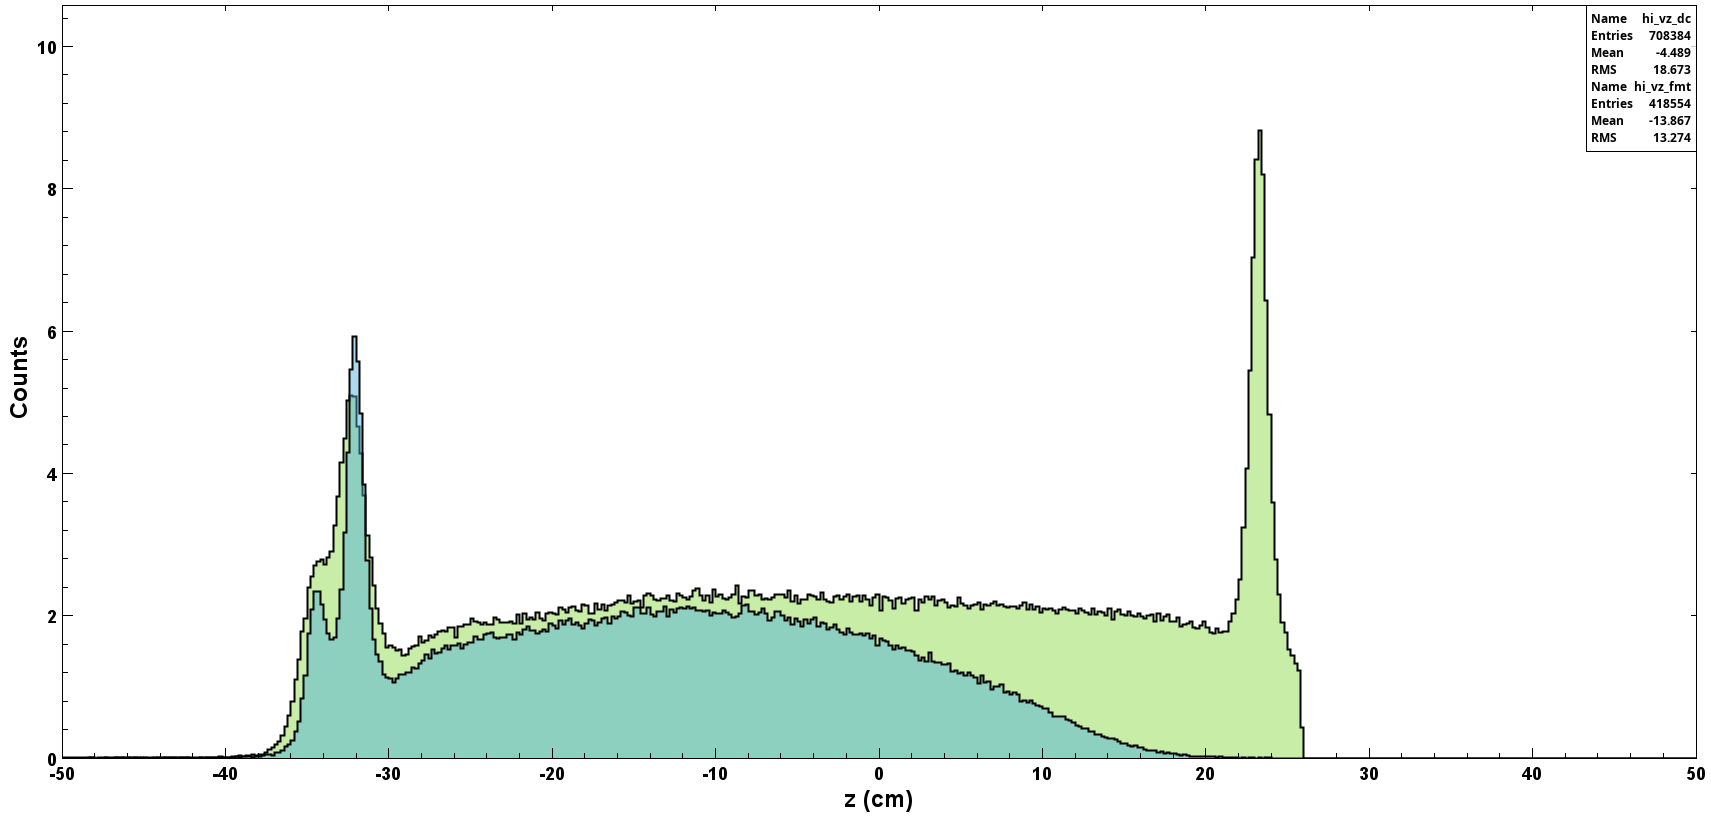
\includegraphics[width=\textwidth]{41dc_vs_fmt.png}}
        \caption[DC vs FMT $z$ without geometric correction]{DC vs FMT vertex $z$ for electrons without any geometric correction. DC tracks are shown in green while FMT tracks are shown in blue. Note that the dark cyan colour comes from the overlap.
        Source: \texttt{fmtVertex.groovy} script in \hyperlink{github.com/JeffersonLab/clas12alignment}{CLAS12 alignment software}.}
        \label{fig::12.41::dc_vs_fmt_vz_11983}
    \end{figure}

    Some additional cuts are applied to the tracks to obtain the plots presented in this section.
    These cuts are used to remove very poor tracks that would not be suitable for analysis regardless.
    The applied cuts are as follows:
    \begin{itemize}
        \item
            \texttt{abs(chi2pid) < 5}:
            This cut removes tracks that do not provide sufficient certainty regarding the particle's PID.
        \item
            \texttt{vz < fmtZ}:
            This cut removes tracks located further downstream than the FMT.
        \item
            \texttt{chi2/ndf < 15}:
            This cut excludes tracks with excessively high uncertainty.
    \end{itemize}
